%System Design

\chapter{Design} % Main chapter title
\label{chapter4_d}
This chapter provides a detailed description of the designed system. In section ~\ref{gfd}, the general framework design diagram is presented, along with a simplifying description of each module the diagram contains. In chapter~\ref{app_d} we describe the basic characteristics of the application we developed. Following, we present in detail all framework modules.


\section{Framework Design}
\label{gfd}
\begin{figure}
	\centerline{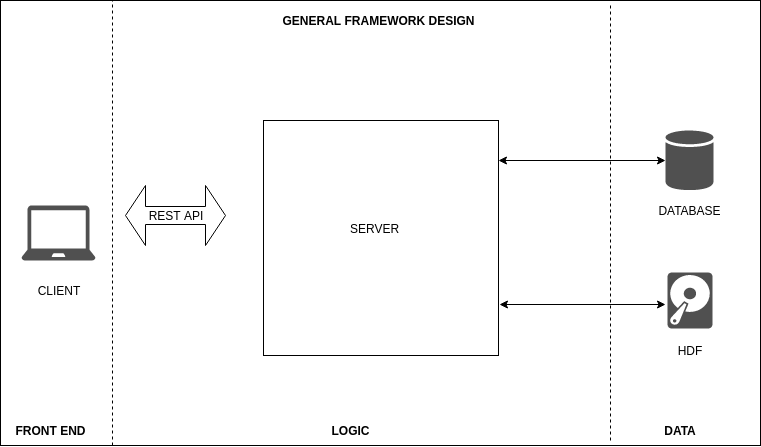
\includegraphics[scale=0.5]{framework.png}}
	\caption{General Framework Design}
	\label{framework}
\end{figure}
In figure~\ref{framework} a general framework design diagram is presented. The system architecture is divided into three parts: front-end/presentation tier, logic tier and data tier, as described in chapter~\ref{3tierarch}. The data tier contains the database where all model data is stored and the filesystem in which all uploaded datasets are saved in hdf file format. The logic tier contains all the modules necessary for ensuring the framework functionality, such as CRUD operations, database access, authentication, authorization etc. The communication between logic and presentation tier is established over a REST API service. In the presentation tier, the user may interact with the server by sending requests and retrieve JSON data as responses. Before we continue in further details about the core system modules,  we describe the basic concepts of the application we created on top of our framework, in order to better demonstrate its capabilities.

\section{Application description}
\label{app_d}
The application makes use of the framework's infrastructure, aiming to present an example of a real use case. Its purpose is to create user networks, which work in common with projects and their data. The data could be text or multi-dimensional datasets. The application utilizes data visualization, aiming to a better understanding and conclusion extraction from the arithmetic datasets. The users may upload their datasets (in hdf file format), in order to make them visible to all the project users, while at the same time they may create plots based on them. In this chapter, we describe the general design of the framework, but we provide some application design details when necessary. The detailed application implementation and functionality is presented in the next chapter.

\section{Framework Modules}
\label{modules}
In this section, the framework modules used in this thesis are presented in detail. Diagrams are shown in some of these subsections for a better understanding of the framework design. The modules are divided into three big categories: NoSQL access, main server and user interface. Each of these modules are a big part of the system's functionality and contain smaller submodules.
	
\section{Model Driven Approach and Module Extensibility}
\begin{figure}
	\centerline{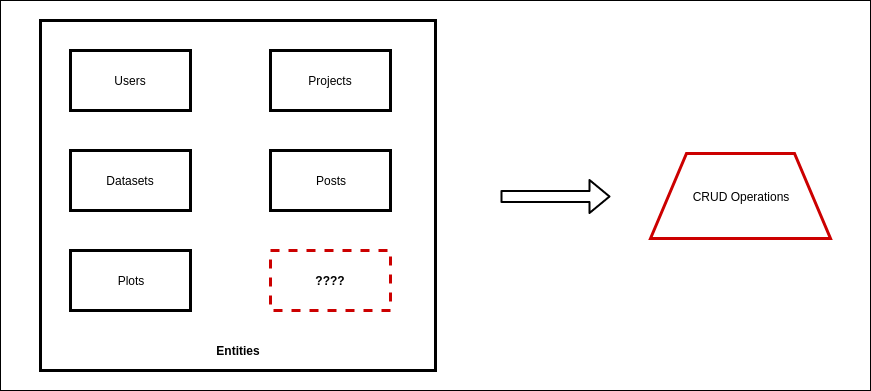
\includegraphics[scale=0.5]{extensible.png}}
	\caption{A group of entities and the generated CRUD operations}
	\label{extensible}
\end{figure}
All modules and submodules are developed in a generic way, are highly customizable, extensible and reusable. This gives us the opportunity to often refer to these modules as models, as described in chapter~\ref{mdsd}. The level of abstraction may change, but the main characteristics of model driven software development are constantly used in the framework implementation. Also, all modules are isolated and expose only the methods that must be used in the rest of the framework. In this way, we ensure that the system modules follow the principles of model driven architecture approach. \par
	The module extensibility is a key feature of the model driven approach. Any extra operation can be added, either within the context of an already developed model or as a new, independent one. Figure ~\ref{extensible} shows an example of a possible module extension while ensuring the development independence from other models. In this example we present a group of entities and the generated CRUD operations. At any moment we may add new entities to the existing group, without breaking the cohesion of the framework. More information about entities can be seen in chapter ~\ref{entities}.

\subsection{NoSQL access}
\label{nosql}
\begin{figure}
	\centerline{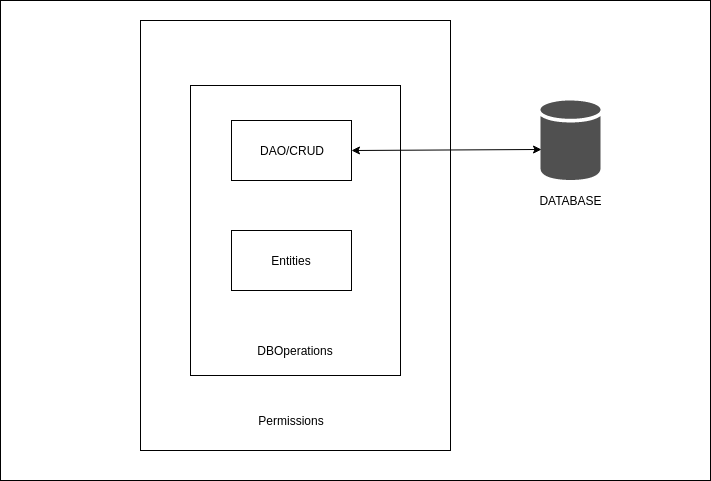
\includegraphics[scale=0.5]{nosqlaccess.png}}
	\caption{NoSQL access module structure}
	\label{nosqlaccess}
\end{figure}
The NoSQL access module is a very important component of the framework. It is responsible for a big part of the system's functionality, such as schema creation, CRUD operations, communication between server and database etc. As a result of its importance, this module is used as a dependency in many other models of the framework. This model is developed in such a way, so that its functionality is isolated from the rest of the framework. In spite of the fact that this practice applies to the model-driven approach, it is generally a neat way for developing frameworks. The structure of the module can be seen in figure ~\ref{nosqlaccess}. NoSQL access module consists of many submodules and each of them is presented separately below. 

\subsubsection{Entities}
\label{entities}
\begin{figure}
	\centerline{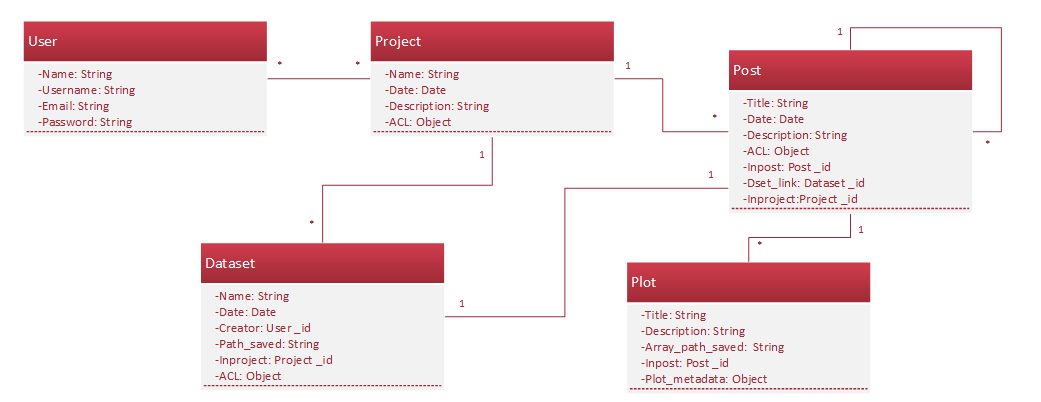
\includegraphics[scale=0.5]{backend.png}}
	\caption{Back end class diagram}
	\label{backend}
\end{figure}
An entity is a representation of a database resource. The creation of an entity through our framework corresponds to the creation of a collection in our database. Likewise, the creation of an instance of an entity, corresponds to the creation of a document inside a collection in our database. In this way, it becomes very easy to make changes to the database, without having direct access to it, which is crucial for our framework.\par
	In the entities module, we define the resources to be used in the framework. More specifically, we define the structure of the entities we use, their fields, their fields type, as well as the fields restrictions. For example, we can specify if a field must be unique in relation to the rest of the instances in the same collection of the database. The definition of the entities is developed in JSON form, therefore it becomes really easy to change or add more entities in the database. So, this module obtains the property of extensibility, which is quite important for the model-driven architecture we developed. \par 
	For the purpose of the application demo, we set a list of entities with specific fields, field types and restrictions. A visualization of this list is shown in figure ~\ref{backend}. An analysis of each of the entities can be seen below.\par
	
	 
\paragraph{Users}
In order to use the application, a user is obliged to create a new user account. The necessary properties to create a new account are a username, full name, password and email. Username and email must have unique values in relation to all other user instances. The user entity  contains all necessary fields to save the above information, along with a unique id.
\paragraph{Projects}
A basic concept of the application is the project entity. The application users may create new projects, in which multiple users may participate. The content of a project is visible for all users that participate in it. The required fields for the creation of a project instance are name, date and description. The project entity uses the concept of ACL, as described in chapter~\ref{acl}. Thus, project entity contains information concerning the users which have access to modify a specific instance of the project entity. In this way, the fields that contain this information refer to an instance of a user entity.
\paragraph{Datasets}
Another valuable entity of the application is Datasets. The application users may create their own datasets inside a project they participate. This entity stores the metadata information of the HDF files which are uploaded on the application. The fields of this entity are the dataset name, date, an id that refers to the instance of the user who creates the entity, and the hdf filename. Additionally, saving the project id of the corresponding instance, in which the dataset is in, is required. Finally, just as in project entity, information about the access control list of the dataset, is retained.
\paragraph{Posts}
An application user may create a new post inside a project. The required fields for the creation of a post entity are title, description, date, a dataset instance reference and a project instance reference. Furthermore, ACL information  is saved in the post entity instance. The user may create a post in response to another post. In this case, information about the post instance in reference is retained.
\paragraph{Plots}
A user may add plots inside his posts. The required fields for the creation of a plot entity are title, description, the path inside the HDF file in which the array used for the plot is saved, and the post instance reference. Finally, the plot entity retains information about its metadata, such as plot type and the dimension values used in the plot.

\subsubsection{Data Access Object/ CRUD}
\label{daocrud}
As described in chapter~\ref{dao}, DAO provides some specific data operations without exposing details of the database which are not needed. In our case, the DAO model ensures that it is the only module with access to the database, and exposes only the information and CRUD functions which are vital for the rest of the framework. The DAO module is developed in a generic way and it is customizable by the entities module. Thus, for each of our entities, we generate CRUD operations for interaction between the specific database model and the framework. The CRUD methods used in the DAO module are described in detail below.

\paragraph{createItem}
The method createItem is responsible for the creation of new instances of an entity. It receives an object as an argument, it converts it in model instance form and then it saves it. If an error occurs, it returns a new error object. Based on the single responsibility principle, the method does not control the kind of data that are about to be saved.
\paragraph{readItems}
The method readItems is used to read data from the database. It receives a query object as an input. The result, successful or not, is returned as an array object. If an error occurs, it returns a new error object.
\paragraph{updateItem}
The method updateItem is responsible for updating an existing object in the database. To achieve that, it receives as arguments a query object and an object with the new property values. If found, the object is replaced and returned. If an error occurs, it returns a new error object.
\paragraph{deleteItem}
The method deleteItem is used to delete an existing document from the database. It receives a query object as an input, and if the document is found, the method deletes it from the database. If an error occurs, it returns a new error object.

\subsubsection{DbOperations}
As mentioned in the section~\ref{daocrud}, the DAO module is responsible for interacting with the database. The model methods are interacting with the database, perform direct changes and may return a result where applicable. But is there a way to guarantee the integrity of our operations in live data? Throughout our study, we determined that all functions must be wrapped in functions responsible for the verification and validation of the requested data mutation. So in essence, we provide a single sandboxed environment securing the database from malicious adversaries, as well as potential internal misuse. \par 
	The DbOperations model was developed for this purpose. It receives as an argument the entities and the DAO models. The DbOperations model returns a group of functions which control the data they receive as an input and then call the corresponding DAO model methods. \par 
	The verification of the data is essential for the CRUD operations. In our case we primarily check if all the required properties and references are contained in the input object. Then, we verify that the references values are valid ids of the corresponding entities instance. In order to achieve that, the necessary read operations in the database are made.
	
\subsubsection{Permissions}
In chapter~\ref{entities}, we described that most of the entities contain some fields that are responsible for the access control list. To be able to alter these fields in relation to users who can access or not a resource, we developed a module specialized for this task. This module contains some functions which implement the ACL functionality. The dependencies of permissions model are entities and DbOperations models. \par 
	The Permissions module defines all the roles the framework uses. At anytime we can add or remove a role, therefore the model-driven design approach is implemented. This model is also responsible for the verification of the changes that it is about to make. The module exposes only the desired methods so that any unwanted functionality is isolated. The generic methods we developed are described below. 

\paragraph{addUserRole}
This method adds a specific role to a user for the given resource. It receives four arguments as an input, the user id, the object id, the role and the model name. All arguments are verified before proceeding with the entity instance update.
\paragraph{removeUserRole}
RemoveUserRole is a method that does the opposite of the addUserRole. It removes from a user a certain role of a resource. It also receives the same arguments as an input. All arguments are verified before proceeding with the entity instance update.
\paragraph{isAllowed}
This method is the core of the ACL logic. Its purpose is to check if  a user has the permission to perform a CRUD operation in a resource instance. To accomplish that, this method checks if a user id is contained in the model instance of the resource id, which is given as an input. If its not found, the same check is performed in the parent model instance, if it exists. \par 
	The reason behind this extra check is that the parent model instance may have been given a default order which applies for every kid model instance. This operation has the advantage of the reduced database operations, since we don't have to check the access permission of -usually many- users, each time we create a new kid model instance. On the contrary, we set a general rule which applies in all cases, unless it is overridden by another permission access. \par
	An example of this functionality is the creation of a post inside of a project. One way to apply for permission access, is to add all user ids which have read permission for the post, inside its instance. It is preferable though, to set a general rule inside the project which states that, all users who have read access to this project, have also access to its posts.

\paragraph{isAllowedCreate}
IsAllowedCreate has the same functionality as isAllowed method, but it focuses exclusively on create operation, which has slightly different functionality than the rest of the CRUD operations.

\subsection{Main server}
\begin{figure}
	\centerline{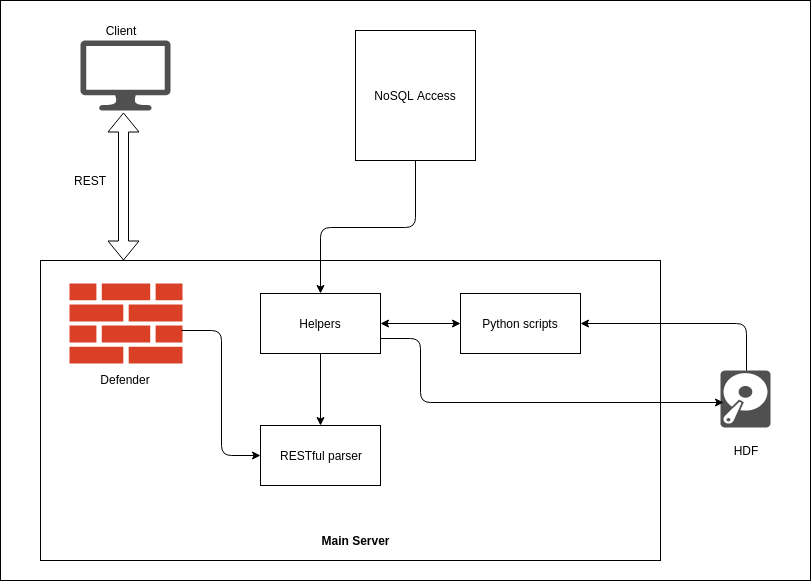
\includegraphics[scale=0.5]{mainserver.png}}
	\caption{Main server module structure}
	\label{mainserver}
\end{figure}
In this section we describe the core framework's component.  The structure of this module can be seen in figure ~\ref{mainserver}. To achieve that, we present all the submodules that are used in this model, and combined together are creating its complete functionality. Thus, apart from routes module which is responsible for receiving requests and sending responds to the client, it is also described the helpers module, which contains a list of functions necessary for this model. Additionally, in this chapter we present a python bridge model, which is used for the utilization of the hierarchical data format, as well as our error handling model, our session setup module and the defenders module. Next, we describe each of these modules.

\subsubsection{Route Handlers}
\label{helpers}
In chapter~\ref{nosql} we defined a list of methods which are responsible for the communication with the database. In order to implement the framework's functionality though, it is necessary to combine these methods into a higher level module. The Route Handlers model is developed for this reason and receives the NoSQL access module as an argument. Also, this module has a dependency on a list of python files, which are vital for the retrieval of saved HDF files (HDF explained in chapter~\ref{hdf}). The returned result of this module's methods is the one that is sent to the client. \par
	Subsequently we present some of these functions. Most of them are developed in conjunction with the application demo, but the module is extensible for any usage. We will skip the functions which are related to the python files. When the python module's purpose is explained, we will return to present the corresponding functions.

\paragraph{saveData}
The function saveData is used for saving an uploaded HDF file in the filesystem. The uploaded file is divided into chunks of data, if it exceeds a specific limit of size. Initially, the method checks if the extension of the file is .h5, and then it collects all the chunks and concatenates them. When the reconstruction of the HDF file is completed, the file is renamed with a unique name and is saved in a specific path inside the filesystem. Then, the function returns the new file name, so that it can be saved in the Dataset entity later. In case an error occurs in the parsing state, an error object is returned.


\paragraph{searchRelatedPosts}
As explained in section ~\ref{entities}, in the context of the application, a post may be created in response to another post. We define a parent post as a post that does not come in response to another post, and a kid post as a post that comes in response to another post, respectively. This function receives as an argument a post id and is searching all the post instances for related posts, kids or parent. The result object of posts is returned in chronological order, ready to be sent to the client.

\paragraph{confFunctions}
confFunctions is a group of methods which are used for the proper configuration of the corresponding objects. It is usual that some of the properties an object contains must be removed before the object is sent to the client. For example, a project entity instance does not need to contain the ACL property, if it is intended to be sent to the client. Thus, these functions remove the unnecessary properties from the corresponding objects. If an error occurs, an error object is returned.

\paragraph{errorHandler}
The framework's error handling, concerning the back end side of the system, sends all possible errors to the errorHandling function. This function categorizes the error and selects a relevant error status and message. Then, the function sends the response object to the client.
	
\subsubsection{Python files}
\label{pyfiles}
Some of the functions that are contained in the route handlers module are dependent on a python model, which includes a list of python modules. In this section we explain the functionality of these modules, and leave the node.js- python communication for the implementation section. \par 
	In general, the python modules are used for the interaction with the HDF files. As explained in chapter ~\ref{hdf}, the hdf contains multidimensional datasets that are saved in a binary format in the filesystem. But in order to make use of this data, we must first convert it from this binary format into floats. The purpose of the python modules is to accomplish exactly that. We present each of these modules below.
	
\paragraph{getHDFContent}
This python script is searching for all dataset arrays inside an HDF file, and returns their metadata. The script receives the name of the HDF file as an argument. Then the function recursively searches all the possible paths inside the file and locates the datasets. The module retains information about each dataset name, shape, size and number of dimensions. This metadata info is crucial for the framework, and it's necessary for its functionality.

\paragraph{getHDFArray}
This script is responsible for returning a chunk of a specific dataset. In order to do that, the module receives a number of arguments, such as the array path, and some state properties. These are used to specify which part of the -usually big- dataset, must be returned. Also, if the dataset is three-dimensional, an extra parameter is sent to declare which dimension's value is to be used.

\paragraph{getHDFPlot}
The last script is developed to return a chunk of a dataset which is presented in a plot. It is similar to the getHDFArray script, with the exception of the zoom functionality and the sampling method. In the getHDFPlot module, a maximum size of a chunk is defined, and based on that, a sampled part of the requested dataset is returned. If the dataset is small in comparison with the maximum size of a chunk, the sampling frequency is high. In another case, the sampling frequency is low. \par 
	The problem with this method is that if the sampling frequency is low, it is impossible to detect details of the dataset. Thus, extra parameters are included, that determine which  part of the dataset must be returned.
	
\paragraph{}
In route handlers module a list of functions, which use the python model, is defined. Thus, the route handlers model is dependent on the python model we described. The basic functionality of these methods is to call the python scripts, parse their results and return it to the next function, respectively. These functions also check for errors that may occur in the python scripts. 


\subsubsection{Routes}
This module is almost exclusively responsible for the communication between server and clients. It's the model which receives the request, distributes it in the corresponding operation and sends the final result back to the client. The routes model implements the RESTful parser, as described in chapter ~\ref{rest}. It includes all the routes which are crucial for the framework's functionality. The model is a requirement of many other modules, such as defender, session, the noSQL access module, route handlers etc.\par
Routes module combines different operations to achieve its own functionality. The core requirement module is the route handlers, from which it receives the result that is in many cases ready to be sent to the client. Routes is a middleware module, meaning that it mediates in the execution of every request between itself and the respond object that is about to be sent to the user. Furthermore, the defender model is a middleware module which precedes the execution of the routes module, and is analyzed below.

\subsubsection{Defender}
\label{def}
The defender module is responsible for the authentication and authorization of the framework's users. Because of the model's middleware functionality, for each request the server receives, the defender module is executed to ensure the framework security. In order to achieve that, the system checks if the user who sent the request is identified, a procedure which is called authentication. Then, the framework implements an authorization check, that is to check if the same user is allowed to send the current request. In case that any of the above operations are not successful, the user access in the system is denied. \par
	The authentication process, although vital for the system, comes at a great cost, because of the constant user identification check with the database. Thus, the framework implements the session management through cookie parsing. During that process, the user logs in the system for the first time, and then receives a cookie which contains all his credential information. From then on, in each future request, the user sends back the cookie in the framework for identification. In this way, the system ensures both security and low cost in database access.


\subsection{User interface}
Up until now, we have only examined the back end module of the framework. The user interface module is the front end layer of the three-tier architecture, as described in chapter ~\ref{3tierarch}. The addition of this module in the already described framework functionality, completes the architecture component which is related to the communication between server and client. \par
	The user interface module is developed in such a way, that it implements the single page application architecture (see chapter~\ref{spa}). This means that in the initialization of the communication between server and client, the client receives all the required resources for the framework operation. These include all the web complaint resources, including HTML5,CSS3 and javascript. From this point on, there is no page reload or further code execution. Furthermore, this model implements the model-driven approach, and that's the reason the developed components are extensible and reusable. We deepen in the front end's implementation in the next chapter.


	